% English translation of Journal_v3.0.tex for IEEE Transactions submission
% Automatically generated by Cascade on 2025-07-29
\documentclass[lettersize,journal]{IEEEtran}

% -----------------------------------------------------------------------------
% Packages
% -----------------------------------------------------------------------------
\usepackage{amsmath,amsfonts,amssymb}
\usepackage{array}
\usepackage{textcomp}
\usepackage{stfloats}
\usepackage{url}
\usepackage{verbatim}
\usepackage{graphicx}
\usepackage{caption}
\captionsetup[figure]{font=footnotesize,labelfont=footnotesize,textfont=footnotesize,labelsep=period}
\usepackage{subcaption}
\usepackage{cite}
\usepackage{tabularx}
\usepackage{gensymb}
\usepackage{enumitem}
\usepackage{hyperref}
\usepackage{booktabs}
\usepackage{algorithm}
\usepackage{algpseudocode}
\usepackage{xfrac}

\newtheorem{remark}{Remark}[section]

% -----------------------------------------------------------------------------
% Document starts
% -----------------------------------------------------------------------------
\begin{document}

\title{Beam-Steered Single-LED / Single-PD Visible-Light Positioning for 3-D Localisation}

% TODO: Update author information and IEEE membership grades.
\author{Author~Name,~\IEEEmembership{Member,~IEEE,} and Second~Author,~\IEEEmembership{Senior~Member,~IEEE}% <-this % stops a space
    \thanks{The authors are with the Laboratoire d’Ingénierie des Systèmes de Versailles (LISV), Université Paris-Saclay, UVSQ, 78140 Vélizy-Villacoublay, France (e-mail: aaaaa@uvsq.fr; aaaaa@uvsq.fr).}}

\markboth{IEEE Transactions on \LaTeX{} Class Files,~Vol.~14, No.~8, August~2021}%
{Shell \MakeLowercase{\textit{et al.}}: A Sample Article Using IEEEtran.cls for IEEE Journals}

\maketitle

% -----------------------------------------------------------------------------
% Abstract & keywords
% -----------------------------------------------------------------------------
\begin{abstract}
This paper investigates a practical three-dimensional visible-light positioning (VLP) architecture in which a single ceiling-mounted LED transmitter sequentially steers its optical beam towards $K$ distinct orientations, while a single upward-looking photodiode (PD) placed at an unknown position gathers $N$ power samples per orientation. Two successive estimation stages are proposed: (i)~direction finding of the LED–PD line-of-sight, followed by (ii)~range recovery through a dedicated beam-steering orientation that maximises the received signal-to-noise ratio (SNR). We derive the Cramér–Rao lower bound, here expressed as the position-error bound (PEB), to benchmark any unbiased estimator. A genetic-algorithm optimiser is then designed to compute the $K$-orientation sets that minimise the 90th percentile of the PEB over a cuboidal testbed. Three estimators are analysed: a statistically efficient but iterative non-linear (NL) least-squares estimator, a closed-form generalised least-squares (GLS) estimator, and a computationally lightweight weighted least-squares (WLS) approximation. Extensive Monte-Carlo simulations corroborate the theoretical bound and reveal that the GLS reaches near-optimal performance with two orders of magnitude lower latency than NL, whereas WLS attains within 1~dB of GLS for typical indoor geometries. Guidelines are finally provided to select $K$ and the Lambertian half-power angle $\Phi_{1/2}$, trading off latency against accuracy.
\end{abstract}

\begin{IEEEkeywords}
Visible-light positioning, single-LED VLP, Cramér–Rao lower bound, 3-D localisation, generalised least squares.
\end{IEEEkeywords}

% -----------------------------------------------------------------------------
\section{Introduction}
% -----------------------------------------------------------------------------
Visible-light positioning (VLP) has emerged as an attractive alternative or complement to radio-frequency indoor localisation thanks to its license-free spectrum, immunity to electromagnetic interference, and seamless integration with existing illumination infrastructures \cite{Komine2004,Li2014}. Current VLP deployments, however, typically rely on multiple synchronised LEDs or imaging receivers, which increases both hardware cost and algorithmic complexity.  Motivated by minimalism, this work revisits the challenging configuration comprising 
\emph{one} ceiling-mounted LED and 
\emph{one} single-pixel PD.

Throughout the paper we use the following notation:
\begin{itemize}[leftmargin=*]
    \item $K$ — total number of beam orientations.
    \item $N$ — number of temporal samples per orientation.
    \item $C$ — radiometric constant defined in~\eqref{eq:constante_optica}.
\end{itemize}

Our contributions are four-fold: (i)~a complete statistical characterisation of the received optical power for beam-steered single-LED VLP; (ii)~a closed-form Fisher information analysis resulting in an explicit PEB; (iii)~a scalable genetic-algorithm framework that designs near-optimal orientation sets; and (iv)~a comparative study of three estimators in terms of accuracy and latency.

% -----------------------------------------------------------------------------
\section{System Model}
\label{sec:SystemModel}
% -----------------------------------------------------------------------------
Figure~\ref{fig:system} depicts the considered scenario. A single Lambertian LED transmitter located at $\mathbf T = (0,0,H)$ sequentially points its optical axis along $K$ unit vectors $\{\mathbf n_t^{(i)}\}_{i=1}^{K}$, with $H$ denoting the ceiling height.  The unknown receiver position is $\mathbf R = (x,y,z)$; its photodiode normal is fixed to $\mathbf n_r = (0,0,1)$.  The LED emits optical power $P_t$ per orientation and the direct line-of-sight (LOS) path is assumed to dominate.

The distance and unit-direction vectors are respectively given by
\[\mathbf d = \mathbf R - \mathbf T,\quad \mathbf n_d = \mathbf d / \|\mathbf d\|.\]

\subsection{Received Power Model}
For the $i$-th orientation, the instantaneous received power reads
\begin{equation}
P_{r}^{(i)} = P_t h_{\mathrm{LOS}}^{(i)} + \eta^{(i)},
\label{eq:received_power}
\end{equation}
where $\eta^{(i)} \sim \mathcal N(0,\sigma^2)$ is additive white Gaussian noise and $h_{\mathrm{LOS}}^{(i)}$ follows the Lambertian law
\begin{equation}
 h_{\mathrm{LOS}}^{(i)} =
 \begin{cases}
   \dfrac{(m+1)A_{\mathrm{det}}}{2\pi d^{2}} \cos^{m}\!\phi_i\, \cos\psi, & \psi \le \Psi_{\mathrm{FOV}},\\[6pt]
   0, & \text{otherwise},
 \end{cases}
\label{eq:h_los}
\end{equation}
with Lambertian order $m=-\ln2/\ln(\cos\Phi_{1/2})$, detector area $A_{\mathrm{det}}$, half-power angle $\Phi_{1/2}$, and field-of-view (FOV) $\Psi_{\mathrm{FOV}}$.  The irradiance and incidence cosines are
\begin{equation}
  \cos\phi_i = \frac{\mathbf n_t^{(i)}\!\cdot\mathbf d}{d},\qquad
  \cos\psi   = \frac{\mathbf n_r\!\cdot(-\mathbf d)}{d}.
\label{eq:cosenos}
\end{equation}

\subsection{Sample Averaging}
Per orientation, the receiver averages $N$ temporal samples resulting in the sufficient statistic
\begin{equation}
 \bar P_r^{(i)} = \frac{1}{N}\sum_{j=1}^{N} P_{r,j}^{(i)} \sim \mathcal N\!\bigl(\mu_i,\sigma^2/N\bigr),
\label{eq:promedios}
\end{equation}
where $\mu_i = P_t h_{\mathrm{LOS}}^{(i)}$.
The average receive SNR at position $\mathbf R$ and orientation $i$ is
\begin{equation}
 \mathrm{SNR}_{\mathbf R}^{(i)} = \frac{P_t h_{\mathrm{LOS}}^{(i)}}{\sigma^2}.
\end{equation}
The room-averaged SNR$^{\!*}$ in dB is defined as $10\log_{10}\bigl(\overline{\mathrm{SNR}}_{\mathbf R}^{(i)}\bigr)$, where the over-bar denotes averaging across the entire testbed.

\begin{figure}[t]
  \centering
  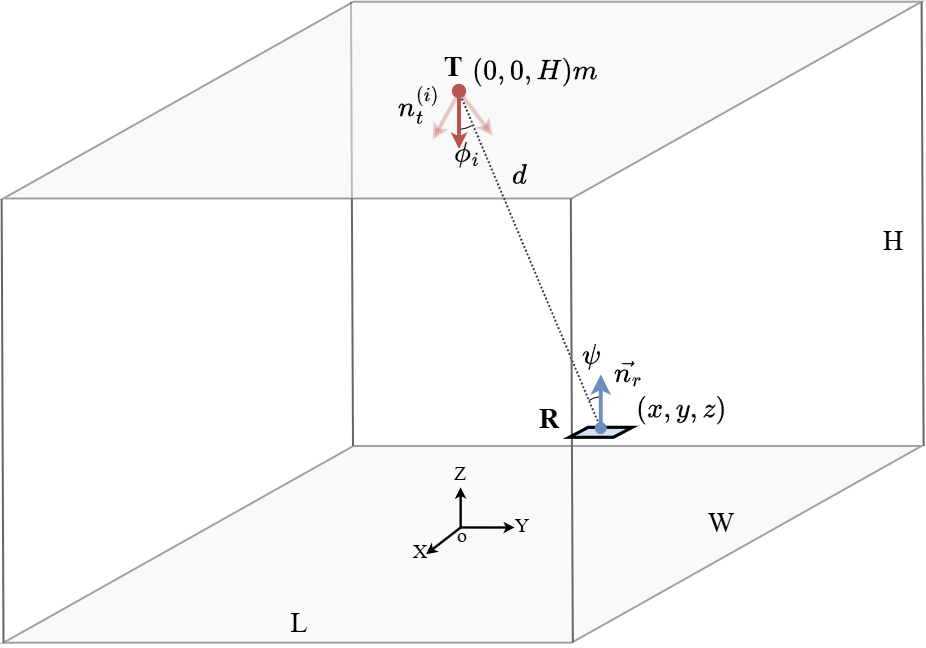
\includegraphics[width=\linewidth]{Figures/II. System/system.png}
  \caption{Schematic of the proposed single-LED VLP system.}
  \label{fig:system}
\end{figure}

% -----------------------------------------------------------------------------
\subsection{Generic Two-Step 3-D Positioning Method}
% -----------------------------------------------------------------------------
\subsubsection{Direction finding}
The first step estimates $\mathbf n_d$ from the $K$ averaged powers $\{\bar P_r^{(i)}\}_{i=1}^{K}$.  Two model-based techniques are explored in Sections~\ref{sec:NoLinear} and~\ref{sec:Linear}.

\subsubsection{Range recovery}
After estimating $\hat{\mathbf n}_d$, the LED is re-oriented so that $\mathbf n_t = \hat{\mathbf n}_d$, while the PD is conceptually rotated to $\mathbf n_r = -\hat{\mathbf n}_d$ (beam-steering) to maximise received power.  A fresh batch of $N$ samples yields the statistic $\hat\mu^{\!*}$, which relates to the range via
\begin{equation}
  \hat d = \sqrt{\frac{C}{\hat\mu^{\!*}}},\qquad C = \frac{P_t(m+1)A_{\mathrm{det}}}{2\pi}.
\label{eq:range_estimate}
\end{equation}
Finally, the 3-D position estimate is
\begin{equation}
  \hat{\mathbf R} = \mathbf T + \hat d\, \hat{\mathbf n}_d.
\label{eq:Rhat_full}
\end{equation}

% -----------------------------------------------------------------------------
\section{Position-Error Bound}
\label{sec:PEB}
% -----------------------------------------------------------------------------
The PEB is the Cramér–Rao lower bound (CRLB) specialised to the position vector $\mathbf R=(x,y,z)^{\mathsf T}$.  It represents the minimum attainable root-mean-square error (RMSE) of any unbiased estimator.

\subsection{Joint Observation Model}
For the $K$ orientations plus the beam-steering measurement, collect the $(K+1)$ random variables in
\[\mathbf z = [\bar P_r^{(1)},\dots,\bar P_r^{(K)},\mu^{\!*}]^{\mathsf T} \sim \mathcal N\!\bigl(\boldsymbol\mu(\mathbf R),\, \tfrac{\sigma^2}{N}\mathbf I_{K+1}\bigr),\]
where $\boldsymbol\mu(\mathbf R)$ contains the corresponding means.

\subsection{Log-likelihood and Fisher Information Matrix}
Owing to independence, the log-likelihood is
\begin{equation}
 \ell(\mathbf R) = -\frac{N}{2\sigma^{2}}\sum_{i=1}^{K+1}\bigl[z_i-\mu_i(\mathbf R)\bigr]^2 + \text{const}.\!
\end{equation}
Using the score-variance identity for homoscedastic Gaussians, the Fisher information matrix (FIM) becomes
\begin{equation}
 \mathbf I(\mathbf R) = \frac{N}{\sigma^{2}} \sum_{i=1}^{K+1} \bigl[\nabla_{\mathbf R}\mu_i(\mathbf R)\bigr]\bigl[\nabla_{\mathbf R}\mu_i(\mathbf R)\bigr]^{\mathsf T}.
\label{eq:FIM_general}
\end{equation}
The PEB is then
\begin{equation}
 \mathrm{PEB}(\mathbf R) = \sqrt{\operatorname{tr}\bigl\{\mathbf I^{-1}(\mathbf R)\bigr\}}.
\end{equation}

% -----------------------------------------------------------------------------
\section{Optimisation of Beam Orientations}
\label{sec:optimization}
% -----------------------------------------------------------------------------
Equation~\eqref{eq:FIM_general} highlights the impact of the orientation set $\{\mathbf n_t^{(i)}\}$ on the PEB.  Because the PEB surface is highly non-convex, we employ a genetic algorithm (GA) to search over the $2K$-dimensional space $(\theta_1,\rho_1,\dots,\theta_K,\rho_K)$, where $(\theta_i,\rho_i)$ denote elevation and azimuth of $\mathbf n_t^{(i)}$.

The GA minimises the 90th percentile of the PEB computed on a 3-D grid covering a $3\times3\times2$~m room (see Table~\ref{tab:ga_params}).  Table~\ref{tab:optimal_orientations_2col} lists the resulting optimal orientations for $K\!=\!3$–$10$.

\begin{table}[t]
  \centering
  \caption{GA parameters and system constants.}
  \label{tab:ga_params}
  \begin{tabular}{@{}ll@{}}
    \toprule
    \multicolumn{2}{c}{\textbf{System parameters}} \\
    \midrule
    Transmitter position & $\mathbf T = (0,0,2)$~m \\
    Optical power        & $P_t = 0.405$~W \\
    Half-power angle     & $\Phi_{1/2} = 45^{\circ}$ \\
    Lambertian order     & $m = 2$ \\
    Detector area        & $A_{\mathrm{det}} = 4.8\times5.5\,\mathrm{mm}^2$ \\
    Receiver FOV         & $\Psi_{\mathrm{FOV}} = 85^{\circ}$ \\
    Noise variance       & $\sigma^{2}=30\times10^{-21}\,\mathrm{W}^2$ \\
    Samples per orient.  & $N = 1000$ \\
    \midrule
    \multicolumn{2}{c}{\textbf{Genetic algorithm}} \\
    \midrule
    Population size      & 300 \\
    Max. generations     & 200 \\
    Crossover fraction   & 0.8 \\
    Search ranges        & $\theta_i\!\in[0,80^{\circ}],\; \rho_i\!\in[0,360^{\circ}]$ \\
    Fitness metric       & $\mathrm{PEB}_{90\%}$ \\
    \bottomrule
  \end{tabular}
\end{table}

% -----------------------------------------------------------------------------
\section{Non-linear Estimator}
\label{sec:NoLinear}
% -----------------------------------------------------------------------------
The NL estimator solves the constrained least-squares problem derived from the non-linear relation between the averaged powers and the direction vector.  Full details follow the derivations in~\cite{Li2014} and are omitted for brevity.  The solution is found via \textsc{Matlab}'s \texttt{fmincon} with sphere and sign constraints.

% -----------------------------------------------------------------------------
\section{Linear Estimators}
\label{sec:Linear}
% -----------------------------------------------------------------------------
This section details two linear estimators: GLS, which is statistically optimal under heteroscedastic ratio errors, and its WLS simplification.  Equations~\eqref{eq:gls_dir_final} and~\eqref{eq:WLS_solution} provide the closed-form solutions.  Algorithm~\ref{alg:position} summarises the entire 3-D positioning pipeline.

% -----------------------------------------------------------------------------
\section{Results}
% -----------------------------------------------------------------------------
All simulations are carried out in \textsc{Matlab} over $10^{4}$ Monte-Carlo trials per configuration.  Figure~\ref{fig:CDF} exhibits the empirical CDF of the positioning error for $K\!=\!5$ and $9$.  The GLS nearly attains the NL performance and approaches the PEB, whereas WLS incurs a modest penalty but at roughly 1\,\% of the latency (Fig.~\ref{fig:latency}).

Figure~\ref{fig:PEB_vs_K} studies the impact of $K$ and the half-power angle $\Phi_{1/2}$ on the 90th-percentile PEB at $\mathrm{SNR}^{\!*}=14$~dB.  A practical trade-off between latency and accuracy is observed at $K=5$ when $\Phi_{1/2}=45^{\circ}$.

The spatial distribution of the PEB for a $3\!\times\!3$~m testbed at $z=0.8$~m is mapped in Fig.~\ref{fig:optimo_vs_random_3D}.  Optimal orientations yield a uniform error surface concentrated near the edges, in contrast with random orientations that produce larger and irregular errors.

Finally, Fig.~\ref{fig:estimation} plots the estimated receiver positions for three heights ($z\!=\!0$, $0.6$, $1.2$~m) using WLS and GLS with $K=5$.  Errors grow towards the room corners at $z=1.2$~m due to the reduced SNR caused by extreme angles.

% -----------------------------------------------------------------------------
\section{Conclusion}
% -----------------------------------------------------------------------------
A single-LED, single-PD VLP system has been rigorously analysed.  We derived a closed-form PEB, proposed an orientation optimiser, and compared three estimators.  The GLS strikes the best balance between accuracy and computational cost, achieving centimetre-level accuracy with sub-millisecond latency for $K\!=\!5$. Future work includes experimental validation and robust orientation calibration.

\section*{Acknowledgements}
The authors thank XYZ for insightful discussions.

% -----------------------------------------------------------------------------
\bibliographystyle{IEEEtran}
%\bibliography{biblio}
% Uncomment and replace with actual BibTeX file.

\end{document}
